\chapter{Trajectory Planning}
\label{cha:trajectory}
For the two most advanced modes, i. e. the Half-Automatic and the Full-Automatic Mode, trajectories had to be generated. In this chapter the best trajectories for \textsc{Skye} are elaborated.

%\subsection{Our Approach}
%From the GUI it was given that the goal trajectory would be a multipoint-interpolating %trajectory. The user is able to define waypoints on a map which afterwards should be %connected with a reasonable and realizable trajectory. Beside interpolating trajectories %there exist also approximating trajectories but they were not taken into consideration, since %usually the user wants skye fly directly through a waypoint.

%In another Bsc Thesis elaborated in this project a controller for waypoint following was %designed. So it was convenient in the scope of this Thesis to use this controller instead of %a specialized trajectory controller.



\section{Definition}
\label{sec:definition}
\subsection{Paths and Trajectories}
\subsection{Interpolation and Approximation}
\subsection{Parametrization}
\subsection{Experimental Design}

\section{Spline Theory}
\label{sec:splineTheory}
references to \cite{engeln}, \cite{biagiotti} and \cite{doessegger}
\subsection{Splines}
\subsubsection{Continuity}
\subsubsection{Boundary Conditions}
\subsubsection{Polynomial Order}
\subsubsection{Parametrization}
\subsection{Piecewise Polynomial Interpolating Splines}
\subsubsection{Boundary Conditions}
\subsubsection{Polynomial Order}
\subsubsection{Parametrization}
\subsection{B-Splines}
\subsubsection{Boundary Conditions}
\subsubsection{Polynomial Order}
\subsubsection{Parametrization}

\section{Trajectory Generation}
\label{sec:trajectoryGeneration}
\subsection{System Constraints}
\subsubsection{Maximum Velocities and Accelerations}
In order to plan a feasible trajectory one has to know the capabilities of the system. Here just a basic derivation for the velocities and accelerations is given, for more details refer to (!!!!Bsc Thesis Joe, Bsc Thesis Andy)\\

The maximum feasible acceleration in any direction is calculated to be:

\begin{equation}
  \left|a_{max} \right| =  \frac{\left|F_{res, w}\right|}{m_{tot}} = 0.96 m/s^2
\end{equation}

Whereas the $F_{res,w}$ is the force resulting from all four thrusters operated under full load in the worst direction and $m_{tot}$ is the sum of the masses of the helium, the virtual mass and the mass of the system itself.\\


The maximum feasible velocity in any direction is calculated to be:

\begin{equation}
\left|v_{max} \right| = \sqrt{\frac{\left|F_{res,w} \right|}{\frac{1}{2}c_d \rho \pi r^2}}=4.7 m/s
\end{equation}

which is nothing but $ \left|F_{res,min} \right| = \left|F_{dray} \right| $.\\

For trajectories for position and orientation the maximal feasible angular acceleration is also important. It is calculated to be:

\begin{equation}
  \left|\Psi_{max} \right| =  \frac{\left|M_{res,w}\right|}{\left| \lambda_{max, J_{B}} \right|} = 2.82 rad/s^2 
\end{equation}

which is quite conservative because it is assumed that worst axis for turning is also the principle axis of the inertia tensor with the highest inertia.\\

Since the system is almost undamped for rotations, the rotational velocities will never be the limiting factor.

\subsection{Time Parametrization}

\section{Controller Implementation}
Some common trajectory controllers are tested to follow the defined trajectories. \textit{Trajectory following} supplies the system's position controller \cite{meier} with a feed forward reference signal. Although it delivers good results for ideal case, the tracking fails if disturbances occure. The \textit{pure pursuit} and \textit{cross track error} controller include an outer feedback loop and are therfore more robust. The \textit{pure pursuit} contoller bases on a path only and therefore yields to worse results compared to the trajectory based \textit{cross track error} controller.
\\ XXXX see \cite{snider} and \cite{deluca}
\label{sec:controllerImplementation}
\subsection{Trajectory Following}
Assuming a perfect model and a trajectory considering all system constraints\footnote{I.e. saturations of $\dot{r}(t)$ and its derivatives.}, the position $r\left(t\right)$ of the system can be assumed to be equal to the trajectory $\tilde{p}(t)$ at any time. Therefore, a straight forward way of a trajectory controller is to follow the trajectory $\tilde{p}(t)$ for every time $t$. This yields accurate tracking in a safe environment \cite{doesegger}.

\begin{equation}
  [r_{ref}(t), \; \dot{r}_{ref}(t), \; \ddot{r}_{ref}(t)]^T = [\tilde{p}(t), \; \dot{\tilde{p}}(t), \; \ddot{\tilde{p}}(t)]^T
\end{equation}

Testing the controller yields good performance.. BLA BLA Graphic figure \ref{fig:trajectoryfollowing}
\begin{figure}[h]
  \begin{minipage}[t]{0.48\textwidth}
%    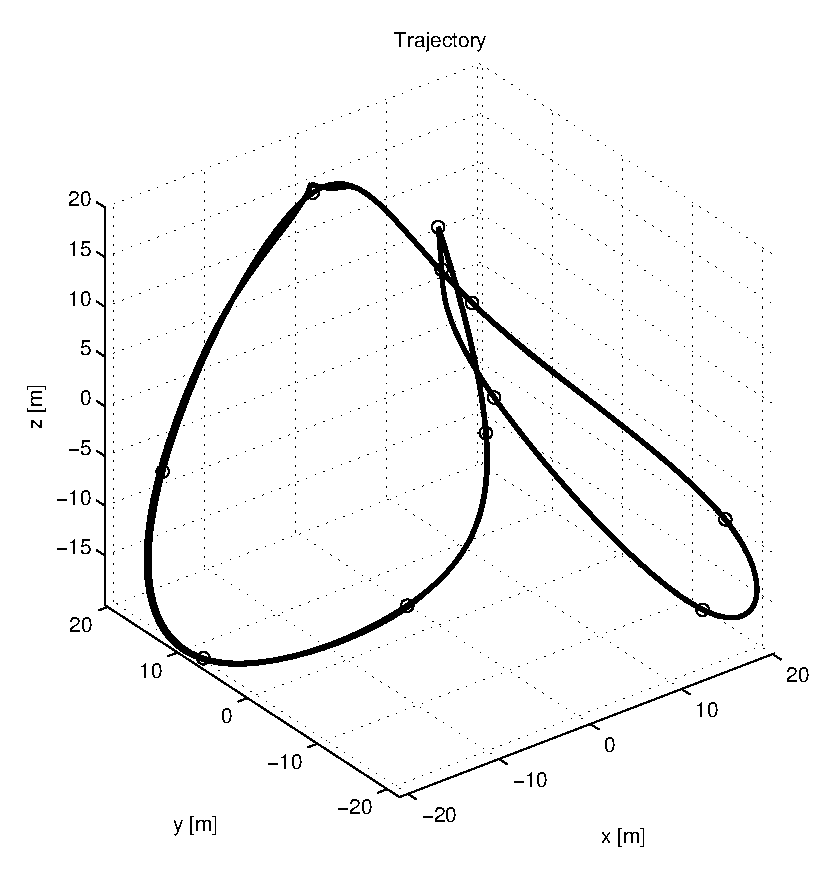
\includegraphics[width = \textwidth]{graphics/a.eps}
  \end{minipage}
  \hfill
  \begin{minipage}[t]{0.48\textwidth}
%    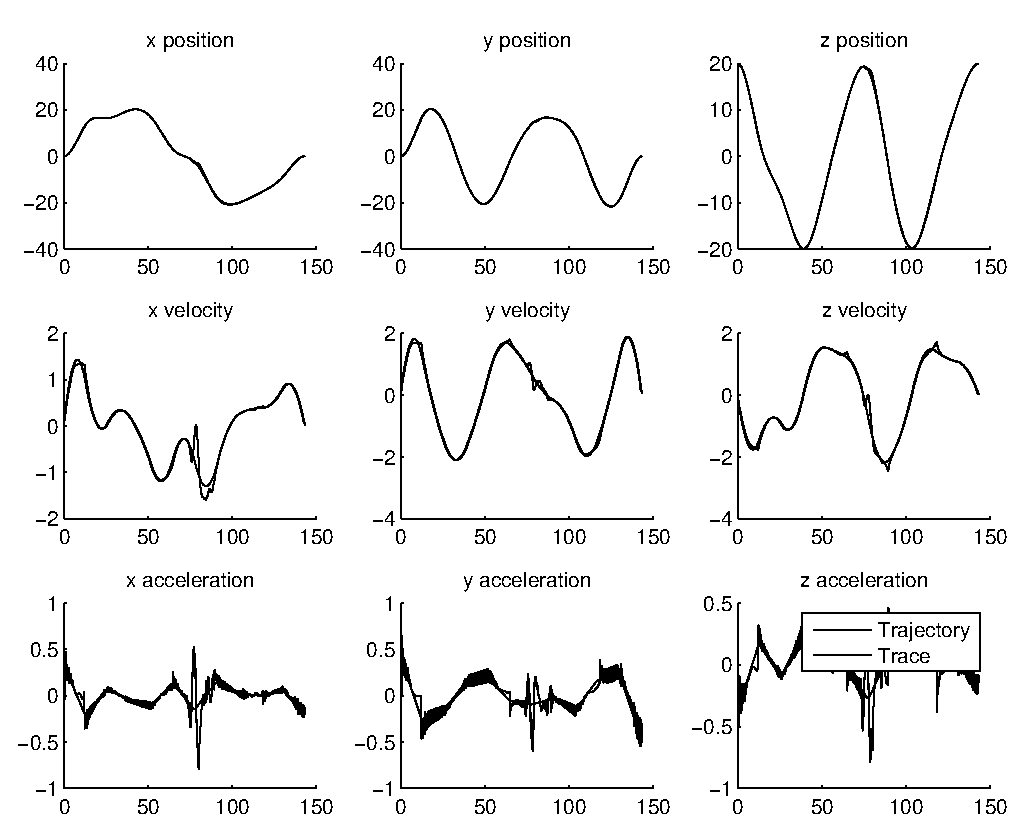
\includegraphics[width = \textwidth]{graphics/b.eps}
  \end{minipage}
  \caption{Trajectory following yields to extremly awesome tracking.}
  \label{fig:trajectoryfollowing}
\end{figure}



\subsection{Pure Pursuit Controller}
Another commonly used trajectory controller is Pure Pursuit \cite{snider}. To consider all dynamics of the trajectory, the reference intput is based on a lookahead point $\tilde{p}(t_{cl+\Delta T}) = \tilde{p}(t_{cl}) + \dot{\tilde{p}}(t_{cl})\Delta T + \ddot{\tilde{p}}(t_{cl}) + ORDNUNG$.
\subsection{Cross Track Error Controller}
see \cite{williams}

\section{Discussion}
\label{sec:discussion}

